\chapter{Le projet Géofibre}
\section{Objet}
Le projet Geofibre a pour objet de fournir une application de SIG pour ORANGE dans le domaine de FTTH\footnote{Fiber To The Home : C'est le réseau trés haut débit de fibre optique pour les clients résidentiels.}.\\
L'application se présente sous la forme d'une page Web permettant de gérer et concevoir des données descriptives du réseau FTTH en France Métropolitaine (\textit{et depuis peu dans les départements d'Outre-Mer}), en temps réel avec plusieurs utilisateurs connectés simultanément.\\
Cette application est principalement destinée aux chargés d'affaire et sous-traitant FTTH.\\
Elle a pour mission, par exemple, de faire évoluer le réseau en permettant la conception sur l'application pour ensuite l'imprimer et l'installer sur le terrain ou par exemple avoir une vision globale des installations sur une commune.\\
En terme de charge, elle comptabilise en 2015 jusqu'a \textbf{1150 utilisateurs simultanés}.\\
Techniquement Geofibre est basé sur le progiciel ArcGIS de l'éditeur ESRI.

\newpage
\section{Historique}
Le lancement du projet a eu lieu en 2010. Jusqu'en 2012 le projet s'est développé dans les locaux du client dans la ville de Lannion suivant la méthode de gestion de projet \textit{AGILE}.\\
Les employés de la société Capgemini étaient à cette époque présents dans les locaux du client pour travailler en tant qu'assistants technique.
Par la suite le développement du projet s'est réalisé dans les locaux de Capgemini, au Spiréa à Rennes.\\\\
Depuis ses débuts Géofibre a évolué de manière significative. \'A l'heure actuelle le projet est à sa 7ème version mineure(cf.\ref{versionning}) et des évolutions sont prévues, d'autant que le gouvernement Français souhaite développer la fibre optique sur l'ensemble du territoire Français.

\section{Illustration}
\begin{figure}[h]
	\captionbox{Capture d'écran du projet Geofibre\label{fig:dummy}}{
		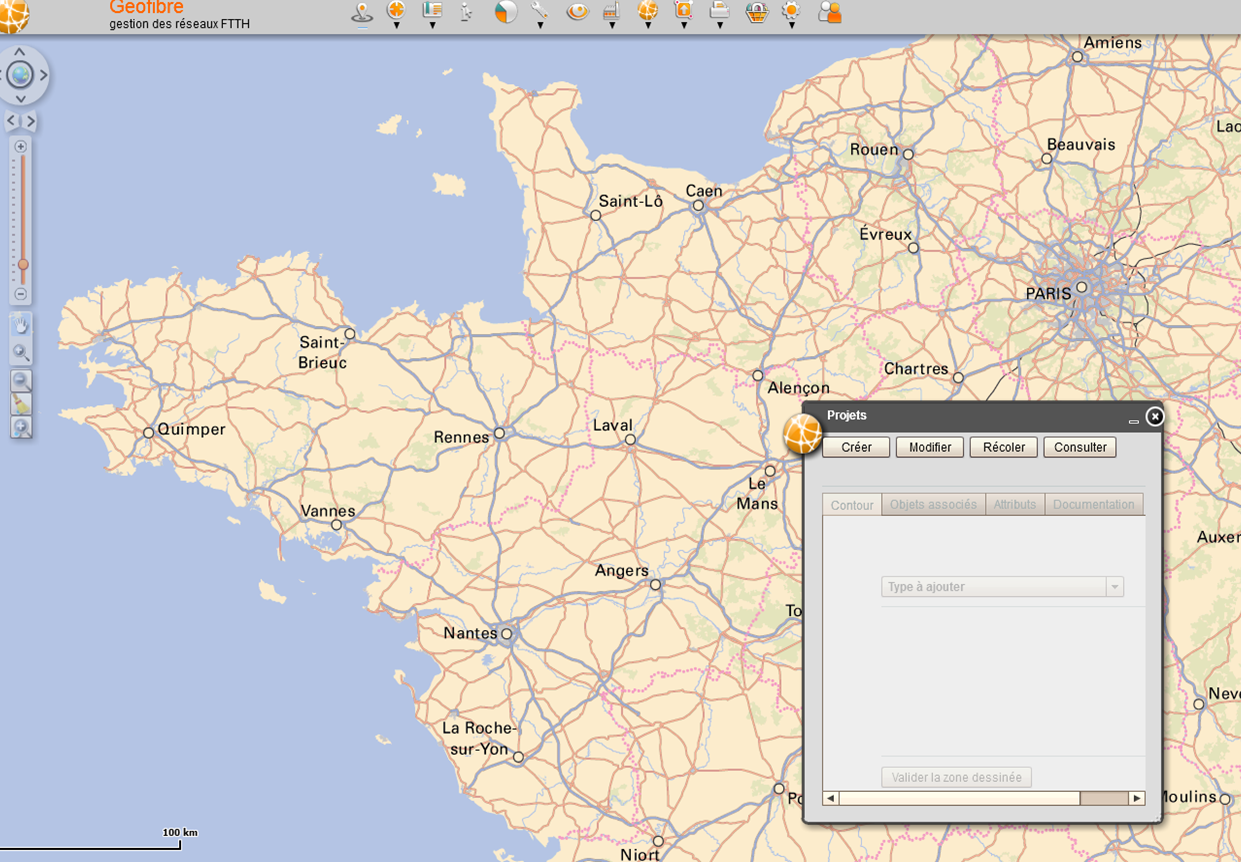
\includegraphics[width=16cm]{images/shotgeofibre.png}
	}
\end{figure}
